% Szglab4
% ===========================================================================
%
\chapter{Analízis modell kidolgozása 1}

\thispagestyle{fancy}

\section{Objektum katalógus}

\subsection{Robot}

A robot objektum felelős azért, hogy tárolja a robot saját pozícióját és sebességét. Ez az objektum képes a pályán olajfoltokat illetve ragacsfoltokat elhelyezni, valamint minden robot tisztában van azzal hogy ezekből mekkora készlet áll még rendelkezésére. Ezen kívül a robotok egyenként ismerik a legfontosabb tulajdonságukat: hogy mekkora távolságot tettek meg már a játék során.

\subsection{Coord}

A Coord objektum Descartes-koordinátákat tartalmaz és visszaadja azokat. Ezen koordináták alapján valósul meg a játék több belső mechanizmusa.

\subsection{Cell}

A cellák tudják magukról, hogy azok most éppen olajfoltosak, ragacsfoltosak, vagy üresek-e, - azaz egyik folt sem található meg rajtuk. A cellák összesége eredményezi a versenyzésre kijelölt pályát. A cellák szabályos sokszög alakúak, minden robot rendelkezik egy kezdőpozícióval, ami egy cellát jelent.

\subsection{Map}

A Map osztály a cellák összeségéből tevődik össze, ezen az objektumon versenyeznek a robotok valójában. A pálya bármilyen alakot felvehet majd. A Map tisztában van azzal, hogy a pályán hol van lyukas cella, s hol nincs. A Map tudja megadni az adott koordinátájú cella szomszédos, üresen álló celláit is. Erre akkor van szükség, ha két robot egyszerre szeretne ugyanarra a cellára ugrani.

\subsection{Game}

A Game objektum köti össze a Robot és Map objektumok működését, . Képes beállítani a játék elején a kezdőértékeket. A játékhoz hozzá tud adni robotokat illetve el tudja távolítani azokat, illetve a léptetést is ez az objektum végzi, ami a játék körökre osztott mivoltát adja. Amennyiben ütközés van a pályán, észleli és lekezeli azokat. 




\section{Osztályok leírása}
% Az előző alfejezetben tárgyalt objektumok felelősségének formalizálása attribútumokká, metódusokká. Csak publikus metódusok szerepelhetnek. Ebben az alfejezetben megjelennek az interfészek, az öröklés, az absztrakt osztályok. Segédosztályokra még mindig nincs szükség. Az osztályok ABC sorrendben kövessék egymást. Interfészek esetén az Interfészek, Attribútumok pontok kimaradnak.}


\subsection{Cell}
\begin{itemize}
\item Felelősség\\
Az osztály felelőssége a játék celláinak a reprezentációja. Ebben az osztályban tároljuk az adott cella koordinátáit a megfelelő koordináta rendszerben, illetve ez az osztály tartalmazza a Cella viselkedését is, ami megszabja hogy hogyan hat a robotra, amelyik rálép.

\item Ősosztályok\\
\comment{Mely osztályokból származik (öröklési hierarchia)}\newline
Object $\rightarrow$ Cell
\item Attribútumok\\
\comment{Milyen attribútumai vannak}
	\begin{itemize}
		\item center: A cella közepének a koordinátáját tárolja
		\item behaviour: A cella viselkedését tárolja
	\end{itemize}
\item Metódusok\\
\comment{Milyen publikus metódusokkal rendelkezik. Metódusonként egy-három mondat arról, hogy a metódus mit csinál.}
	\begin{itemize}
		\item void setCenter(Coord c): Beállítja a cella közepének koordinátáit. Amiket ahhoz fogunk használni, hogy megmondjuk hogy a robot éppen melyik cellában van.
		\item Coord getCenter(): Vissza lehet kérni, hogy hol van a cella közepe.
		q
	\end{itemize}
\end{itemize}

\subsection{Game}
\begin{itemize}
	\item Felelősség\\
	Az osztály felelőssége a Játékban található fő objektumok karban tartása és a játék léptetése, ehhez megfelelően rendelkezik az összes robottal, illetve a játék térképével. Ebből az osztályból minden játékhoz pontosan egy objektum tartozik.
	\item Ősosztályok\\
	Object $\rightarrow$ Game
	\item Attribútumok\\
	\begin{itemize}
		\item robots: Egy Map, ami a játékban található robotokat tárolja a nevükkel együtt.
		\item map: Az aktuális játék pályáját tartalmazó attribútum. Ezen a pályán lépkednek a robotok.
		\item rounds: Ebben az attribútumban köröket tartja nyilván.
	\end{itemize}
	\item Metódusok\\
	\begin{itemize}
		\item Robot[] checkCollission(Robot): Megnézi hogy az aktuális robottal ütközik-e másik robot. Ha igen, akkor visszaadja azoknak a Robotnoknak a Listáját, akik ütköznek.
		\item void resolveCollision(Robot[]): Kap egy listát olyan robotokról amik ütköznek, és eldönti, hogy mi legyen velük. Ha van elég szabad cella, akkor szétdobálja őket, ha nincs akkor pedig mind meghalnak.
		\item void kill(Robot): Eltávolítja a játékból a megkapott Robotot.
		\item Coord[] collectRobotPositions(): Visszaadja a játékban lévő összes Robot pozicióját.
		\item Game(Gamesettings): Az osztály konstruktora, ez a függvény állítja be a kezdeti értékeket, és generálja le a Robotokat a paraméterként kapott GameSettings objektum alapján.
		\item void step(): Ez a függvény lépteti a játékot, itt mozognak a robotok, és itt kezdeményezzük az ütközések feloldását.
		\item Map<String, RobotController> getRobotControllers(): ez a függvény Adja vissza a Robotok irányító interfacet, a lényege az, hogy a játékban lévő robotokból csak annyi látszódjon kifele, amennyi minimálisan szükséges.
		\item void terminate(): Ez a függvény fejezi be a játékot, ha a játékos kézzel állította le a játékot, akkor nem hirdet győztest.
	\end{itemize}
\end{itemize}


\subsection{GameSettings}
\begin{itemize}
	\item Felelősség\\
	Az osztály felelőssége az, hogy azokat az információkat amik egy új játék elkezdéséhez szükségesek egységbe zárja, és így adja át a Game osztály konstruktorának, ami elvégzi az inicializálást.
	\item Ősosztályok\\
		Object $\rightarrow$ GameSettings
	\item Attribútumok\\
	\begin{itemize}
		\item mapFile: A pályát tartalmazó File-ra mutat.
		\item initialSticky: tárolja, hogy a robotok mennyi ragaccsal kezdjenek.
		\item initialOily: tárolja hogy a robotok hány olajfolttal kezdjenek.
		\item rounds: tárolja, hogy a játék hány körből álljon.
		\item robotNames: ebben a listában adjuk át a robotok neveit, és ez implikálja azt is, hogy hány robotot akarunk létrehozni a játékban.
	\end{itemize}
	\item Metódusok\\
	\begin{itemize}
		\item void setMapFile(File): a mapFile attribútumot beállító metódus.
		\item File getMapFile(): A mapFile értékét visszaadó metódus.
		\item void setInitialSticky(int): az initialSticky attribútumot beállító metódus.
		\item int getInitialSticky(): Az initialSticky értékét visszaadó metódus.
		\item void setInitialOily(int): Az initialOily attribútumot beállító metódus.
		\item int getinitialOily(): Az initialOily értékét visszaadó metódus.
		\item void setRounds(int): A rounds attribútumot beállító metódus.
		\item int getRounds(): A rounds értékét visszaadó metódus.
		\item void setRobotNames(int): A robotNames attribútumot beállító metódus.
		\item List<String> getRobotNames(): A robotNames értékét visszaadó metódus.
	\end{itemize}
\end{itemize}

\subsection{Osztály2}
\begin{itemize}
\item Felelősség\\
\comment{Mi az osztály felelőssége. Kb 1 bekezdés.}
\item Ősosztályok\\
\comment{Mely osztályokból származik (öröklési hierarchia)\newline
Legősebb osztály $\rightarrow$ Ősosztály2 $\rightarrow$ Ősosztály3...}
\item Interfészek\\
\comment{Mely interfészeket valósítja meg.}
\item Attribútumok\\
\comment{Milyen attribútumai vannak}
	\begin{itemize}
		\item attribútum1: attribútum jellemzése: mire való
		\item attribútum2: attribútum jellemzése: mire való
	\end{itemize}
\item Metódusok\\
\comment{Milyen publikus metódusokkal rendelkezik. Metódusonként egy-három mondat arról, hogy a metódus mit csinál.}
	\begin{itemize}
		\item int foo(Osztály3 o1, Osztály4 o2): metódus leírása
		\item int bar(Osztály5 o1): metódus leírása
	\end{itemize}
\end{itemize}


\section{Statikus struktúra diagramok}
\comment{Az előző alfejezet osztályainak kapcsolatait és publikus metódusait bemutató osztálydiagram(ok). Tipikus hibalehetőségek: csillag-topológia, szigetek.}

\clearpage

\section{Szekvencia diagramok}
\comment{Inicializálásra, use-case-ekre, belső működésre. Konzisztens kell legyen az előző alfejezettel. Minden metódus, ami ott szerepel, fel kell tűnjön valamelyik szekvenciában. Minden metódusnak, ami szekvenciában szerepel, szereplnie kell a valamelyik osztálydiagramon.}

\begin{figure}[!htbp]
\begin{center}
	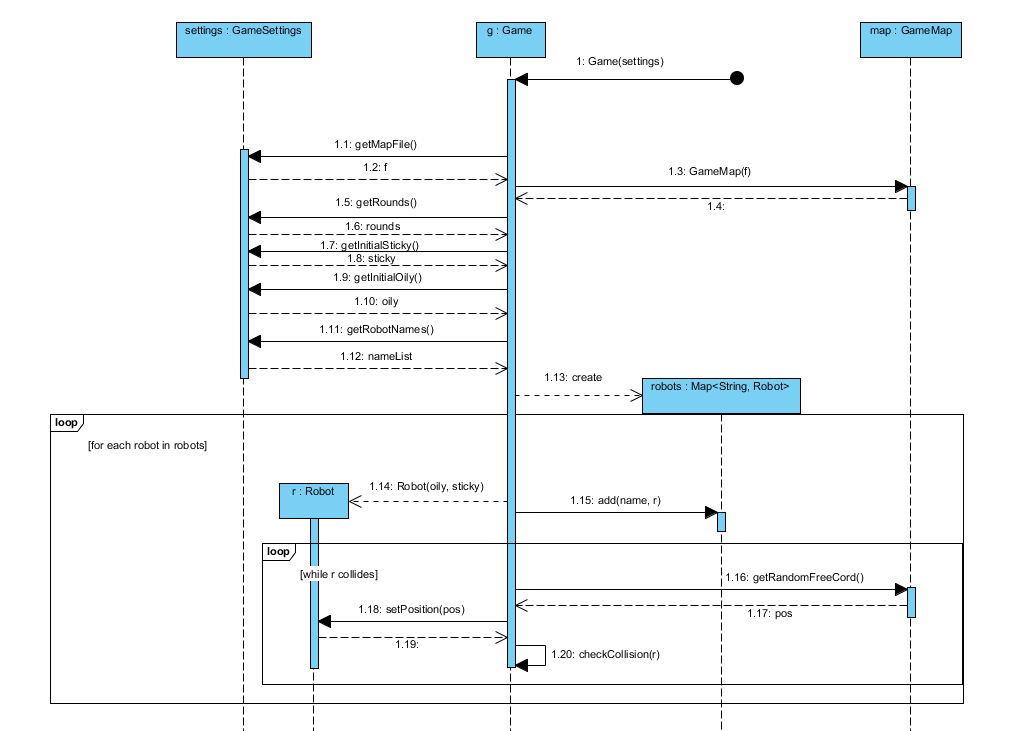
\includegraphics[width=\textwidth, center]{./chapters/chapter03/startgame.png}
	\caption{Játékindítás}
\end{center}
\end{figure}

\begin{figure}[!htbp]
\begin{center}
	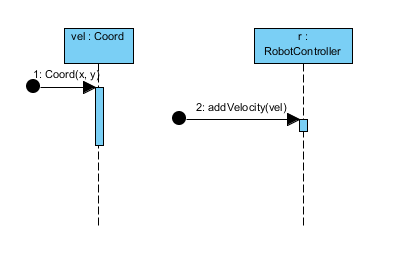
\includegraphics[width=90mm, center]{./chapters/chapter03/velocity.png}
	\caption{Sebességvektor beállítása}
\end{center}
\end{figure}



\begin{figure}[!htbp]
	\begin{center}
		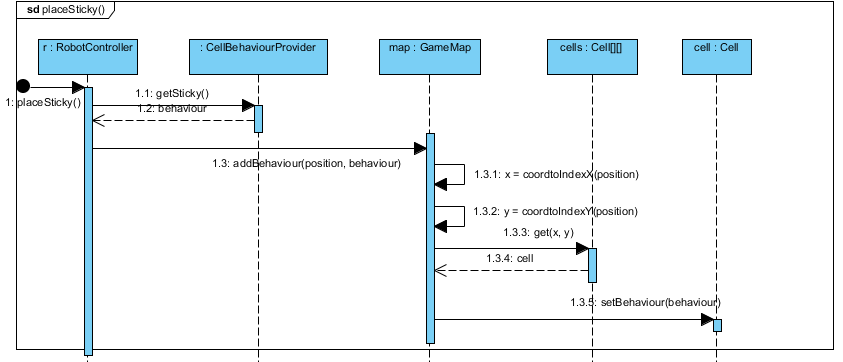
\includegraphics[width=\textwidth, center]{./chapters/chapter03/sticky.png}
		\caption{Ragacs elhelyezése}
	\end{center}
\end{figure}

\begin{figure}[!htbp]
	\begin{center}
		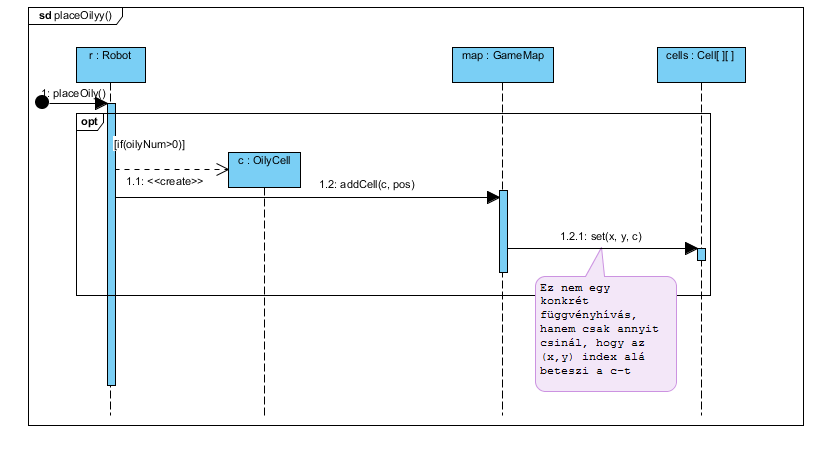
\includegraphics[width=\textwidth, center]{./chapters/chapter03/oily.png}
		\caption{Olaj elhelyezése}
	\end{center}
\end{figure}

\begin{figure}[!htbp]
	\begin{center}
		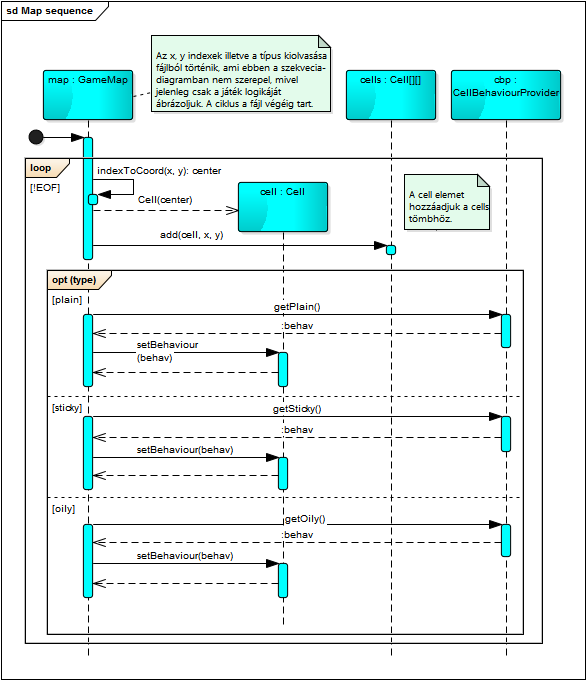
\includegraphics[width=\textwidth, center]{./chapters/chapter03/map.png}
		\caption{Map konstruktorhívása}
	\end{center}
\end{figure}

\begin{figure}[!htbp]
	\begin{center}
		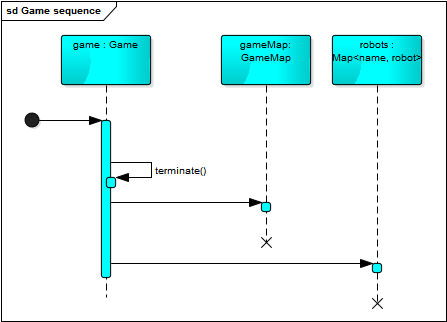
\includegraphics[width=10cm, center]{./chapters/chapter03/endgame.png}
		\caption{Játék vége}
	\end{center}
\end{figure}



\clearpage


\section{State-chartok}
\comment{Csak azokhoz az osztályokhoz, ahol van értelme. Egyetlen állapotból álló state-chartok ne szerepeljenek. A játék működését bemutató state-chart-ot készíteni tilos.}

\begin{figure}[h]
\begin{center}
%\includegraphics[width=17cm]{chapters/chapter03/example.pdf}
\caption{x}
\label{fig:example3}
\end{center}
\end{figure}

